\documentclass{beamer}

\usepackage[utf8]{inputenc}   % Підтримка UTF-8
\usepackage[ukrainian]{babel} % Підтримка української мови
\usepackage[ukrainian=nohyphenation]{hyphsubst}
\usepackage{booktabs}
\usepackage[T2A]{fontenc}      % Кодова таблиця для кирилиці
\usepackage{amsmath, amsfonts} % Для математики, якщо потрібно
\usepackage{hyperref}          % Для створення посилань
\usepackage{listings}          % Пакет для вставки коду
\usepackage{graphicx}
\usepackage{csvsimple}
\usepackage{parskip}
\usepackage{csquotes}
\usepackage{xcolor}
\usepackage{multicol} % Для багатостовпчикового тексту

\usepackage{tabularray}
\usepackage{float}
\usepackage{codehigh}
\usepackage[normalem]{ulem}

\UseTblrLibrary{booktabs}
\UseTblrLibrary{siunitx}
\newcommand{\tinytableTabularrayUnderline}[1]{\underline{#1}}
\newcommand{\tinytableTabularrayStrikeout}[1]{\sout{#1}}
\NewTableCommand{\tinytableDefineColor}[3]{\definecolor{#1}{#2}{#3}}

\usetheme{Madrid}

% Прибираєм навігацію з кожного слайду
\beamertemplatenavigationsymbolsempty

\title{Лабораторна робота №3}
\subtitle{Регресійний аналіз}
\subtitle{Команда №9}

% [], щоб прибрати імена з кожного слайду
\author[]{
  Баранівська В.О.,
  Корсун Є. В.,
  Хмарук О. Ю.,
  Літковський А.С.,
  Кудін Н. А.
}
\date{2025}

\begin{document}

\frame{\titlepage}

\graphicspath{{../../../}} % Ensure this path is correct or remove it if not needed

%Короткий підсумок ЛР 1-2 (якщо є свіжі погляди, можна ще зменшити/додати/змінити)

\begin{frame}
  \section{Набір даних}

  \frametitle{Зміст}
  \tableofcontents[currentsection]
\end{frame}

\begin{frame}
  \frametitle{Набір даних}

  Було вирішено дослідити якість повітря Тайваню. Уряд провінції намагається
  контролювати та покращувати якість повітря. Тому 17 грудня 2017 року була введена
  реформа \textit{Air Pollution Control Action Plan}.

  \begin{center}

  \end{center}
\end{frame}

% Подумав, що напевно в цей раз немає сенсу повторювати, те що було в 2 попередніх лабах
% \begin{frame}
%   \frametitle{Набір даних}
% 
%   Загальний опис датасету:
% 
%   \begin{enumerate}
%     \item Кількість рядків: 5\,882\,208
%     \item Кількість стовпців: 25
% 
%     \begin{itemize}
%       \item Числові: 19
%       \item Факторні: 4
%       \item Дата: 1
%       \item Інші: 1
%     \end{itemize}
%   \end{enumerate}
% \end{frame}

\begin{frame}
  \frametitle{Висновки EDA}
  \begin{itemize}
    \item Загальний рівень AQI по регіонам зменшується, тобто показники покращуються після початку реформи.
    Більш явні зміни очікувано помітні через декілька років після реформи.

    \item Якість повітря змінюється нерівномірно у містах.
  \end{itemize}
\end{frame}

% \begin{frame}
%   \frametitle{Висновки з гіпотез та довірчих інтервалів}
%   \begin{itemize}
%   \item 
%   \item 
% 
%   \end{itemize}
% \end{frame}

\begin{frame}
  \section{Моделювання}

  \frametitle{Зміст}
  \tableofcontents[currentsection]
\end{frame}

\begin{frame}
  \frametitle{Питання для дослідження}

  Як реформа покращення якості повітря вплинула на якість повітря?
\end{frame}

\begin{frame}
  \frametitle{Питання для дослідження}

  Даний набір даних є панельним. Для аналізу будемо використовувати модель з фіксованими ефектами.

  \begin{itemize}
    \item Залежна змінна: AQI
    \item Незалежні змінні: after\_reform\footnotemark, windspeed
    \item Контрольні змінні:  
    \item Фіксовані ефекти: sitename (Назва станції вимірювання)
  \end{itemize}

  \footnotetext[1]{Дорівнює 1, якщо дата спостереження після \textit{17 грудня 2017 року}, 0 в іншому випадку}
\end{frame}

\begin{frame}
  \frametitle{Набір даних}

  Для спрощення моделювання перетворимо початковий датасет таким чином:
  
  \begin{itemize}
    \item Згрупуємо дані за датою (без часу)
    \item Знайдемо медіану в кожній групі в числових змінних
  \end{itemize}

  Таким чином, з набору даних на 5\,882\,208 рядків отримуємо 231\,863 рядків, що значно пришвидшує створення моделі.
\end{frame}

% \begin{frame}
%   \frametitle{Пропущені дані по змінним}
%    
% \end{frame}

\begin{frame}
  \frametitle{Зміст}
  \tableofcontents[currentsection]
\end{frame}

\begin{frame}
  \frametitle{Модель}

  Структурна модель:

   $$AQI \sim \beta_1 \, \text{after\_reform} + \beta_2 \, \text{windspeed} + \alpha $$

  \begin{enumerate}
    \item $\beta_1$: Очікується негативний знак. 
    Метою реформи було покращення якості повітря,
    тому після її впровадження AQI мав би знизитися.

    \item $\beta_2$: Очікується негативний знак. 
    Сильніший вітер зазвичай сприяє кращому розсіюванню забруднювачів, 
    що призводить до зниження AQI (покращення якості повітря).
  \end{enumerate}
\end{frame}

\begin{frame}
  \frametitle{Оцінка моделі}
   
  \begin{table}
    \centering
    \begin{talltblr}[         %% tabularray outer open
    entry=none,label=none,
    note{}={+ p \num{< 0.1}, * p \num{< 0.05}, ** p \num{< 0.01}, *** p \num{< 0.001}},
    ]                     %% tabularray outer close
    {                     %% tabularray inner open
    colspec={Q[]Q[]},
    column{2}={}{halign=c,},
    column{1}={}{halign=l,},
    hline{6}={1,2}{solid, black, 0.05em},
    }                     %% tabularray inner close
    \toprule
    & Model \\ \midrule %% TinyTableHeader
    after\_reformTRUE & \num{-12.261}*** \\
    & (\num{0.710}) \\
    windspeed & \num{-0.507} \\
    & (\num{0.476}) \\
    Num.Obs. & \num{221582} \\
    \bottomrule
    \end{talltblr}
  \end{table}
\end{frame}

\begin{frame}
  \frametitle{Оцінка якості моделей (1)}
  
  Розглянемо вплив поліномів та логаритмів

  \begin{itemize}
    \item $\log(\text{windspeed})$ -- модель 2
    \item $\text{windspeed}^2$ -- модель 3
    \item $\text{windspeed}^3$ -- модель 4
  \end{itemize}
\end{frame}

\begin{frame}
  \frametitle{Оцінка якості моделей (2)}
  
  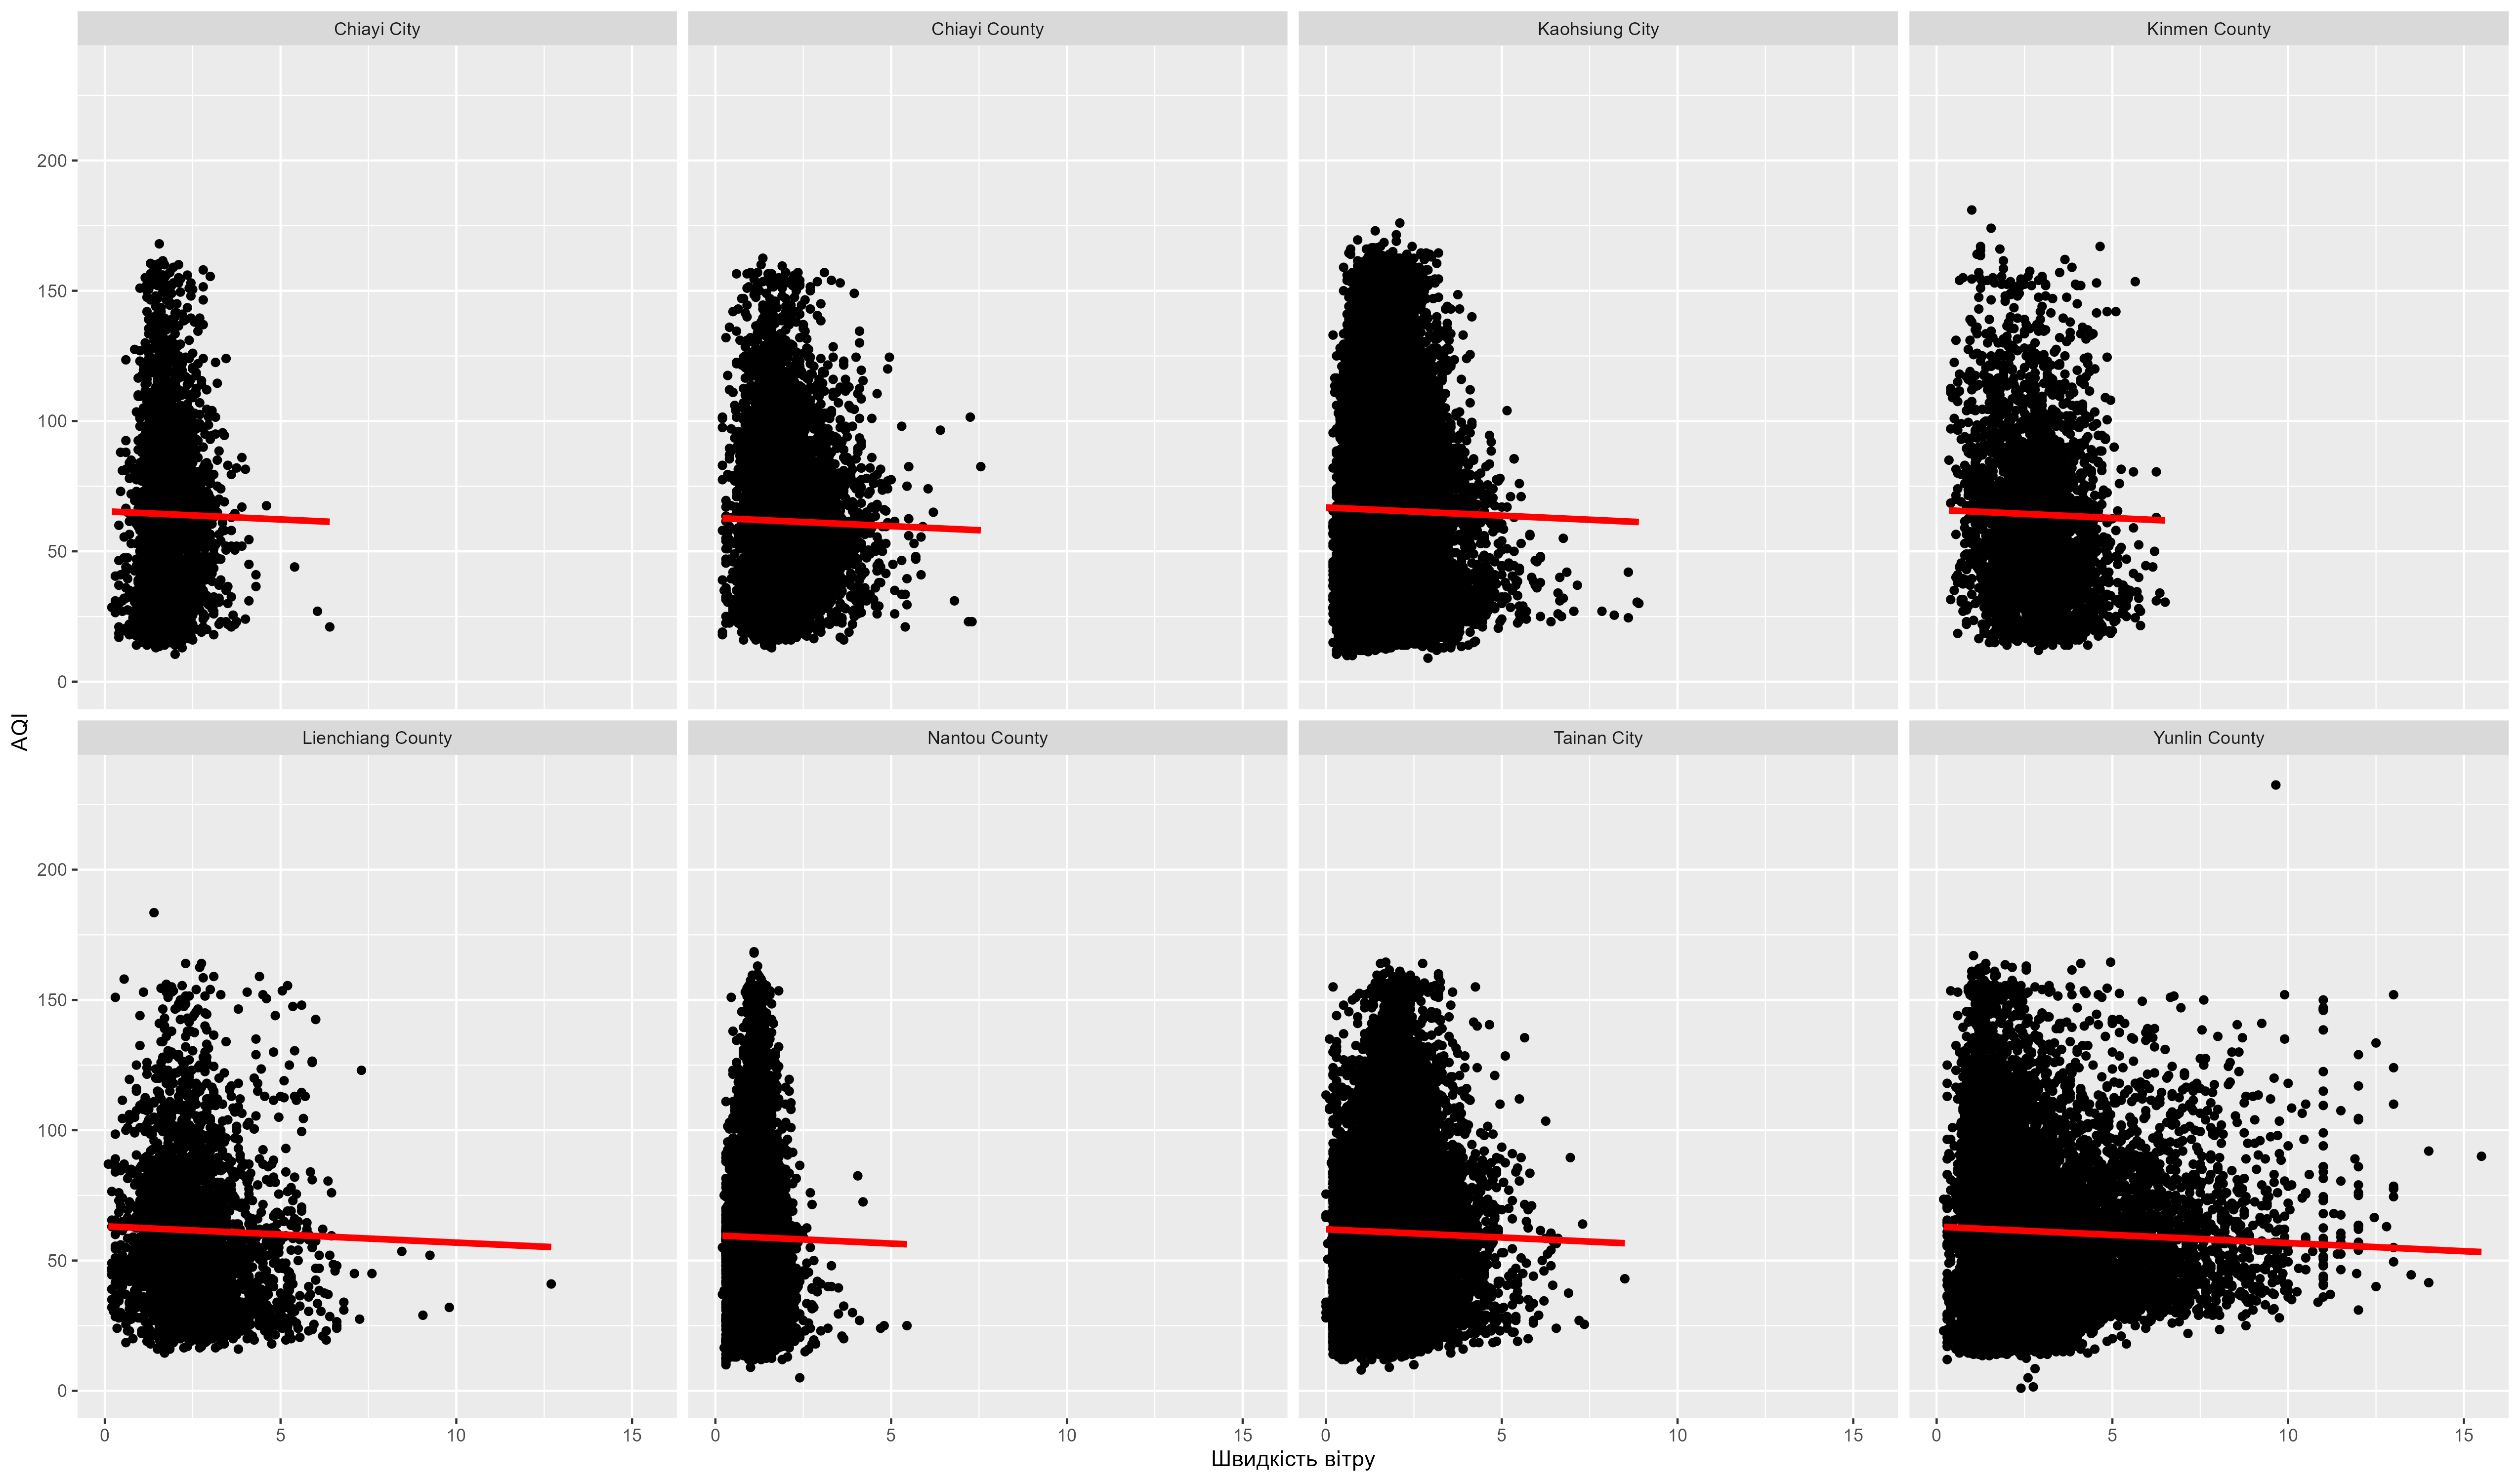
\includegraphics[height=2.8in]{plots/lab3/windspeed-aqi.png}
\end{frame}

\begin{frame}
  \frametitle{Оцінка якості моделей (2)}

  log(windspeed):
  
  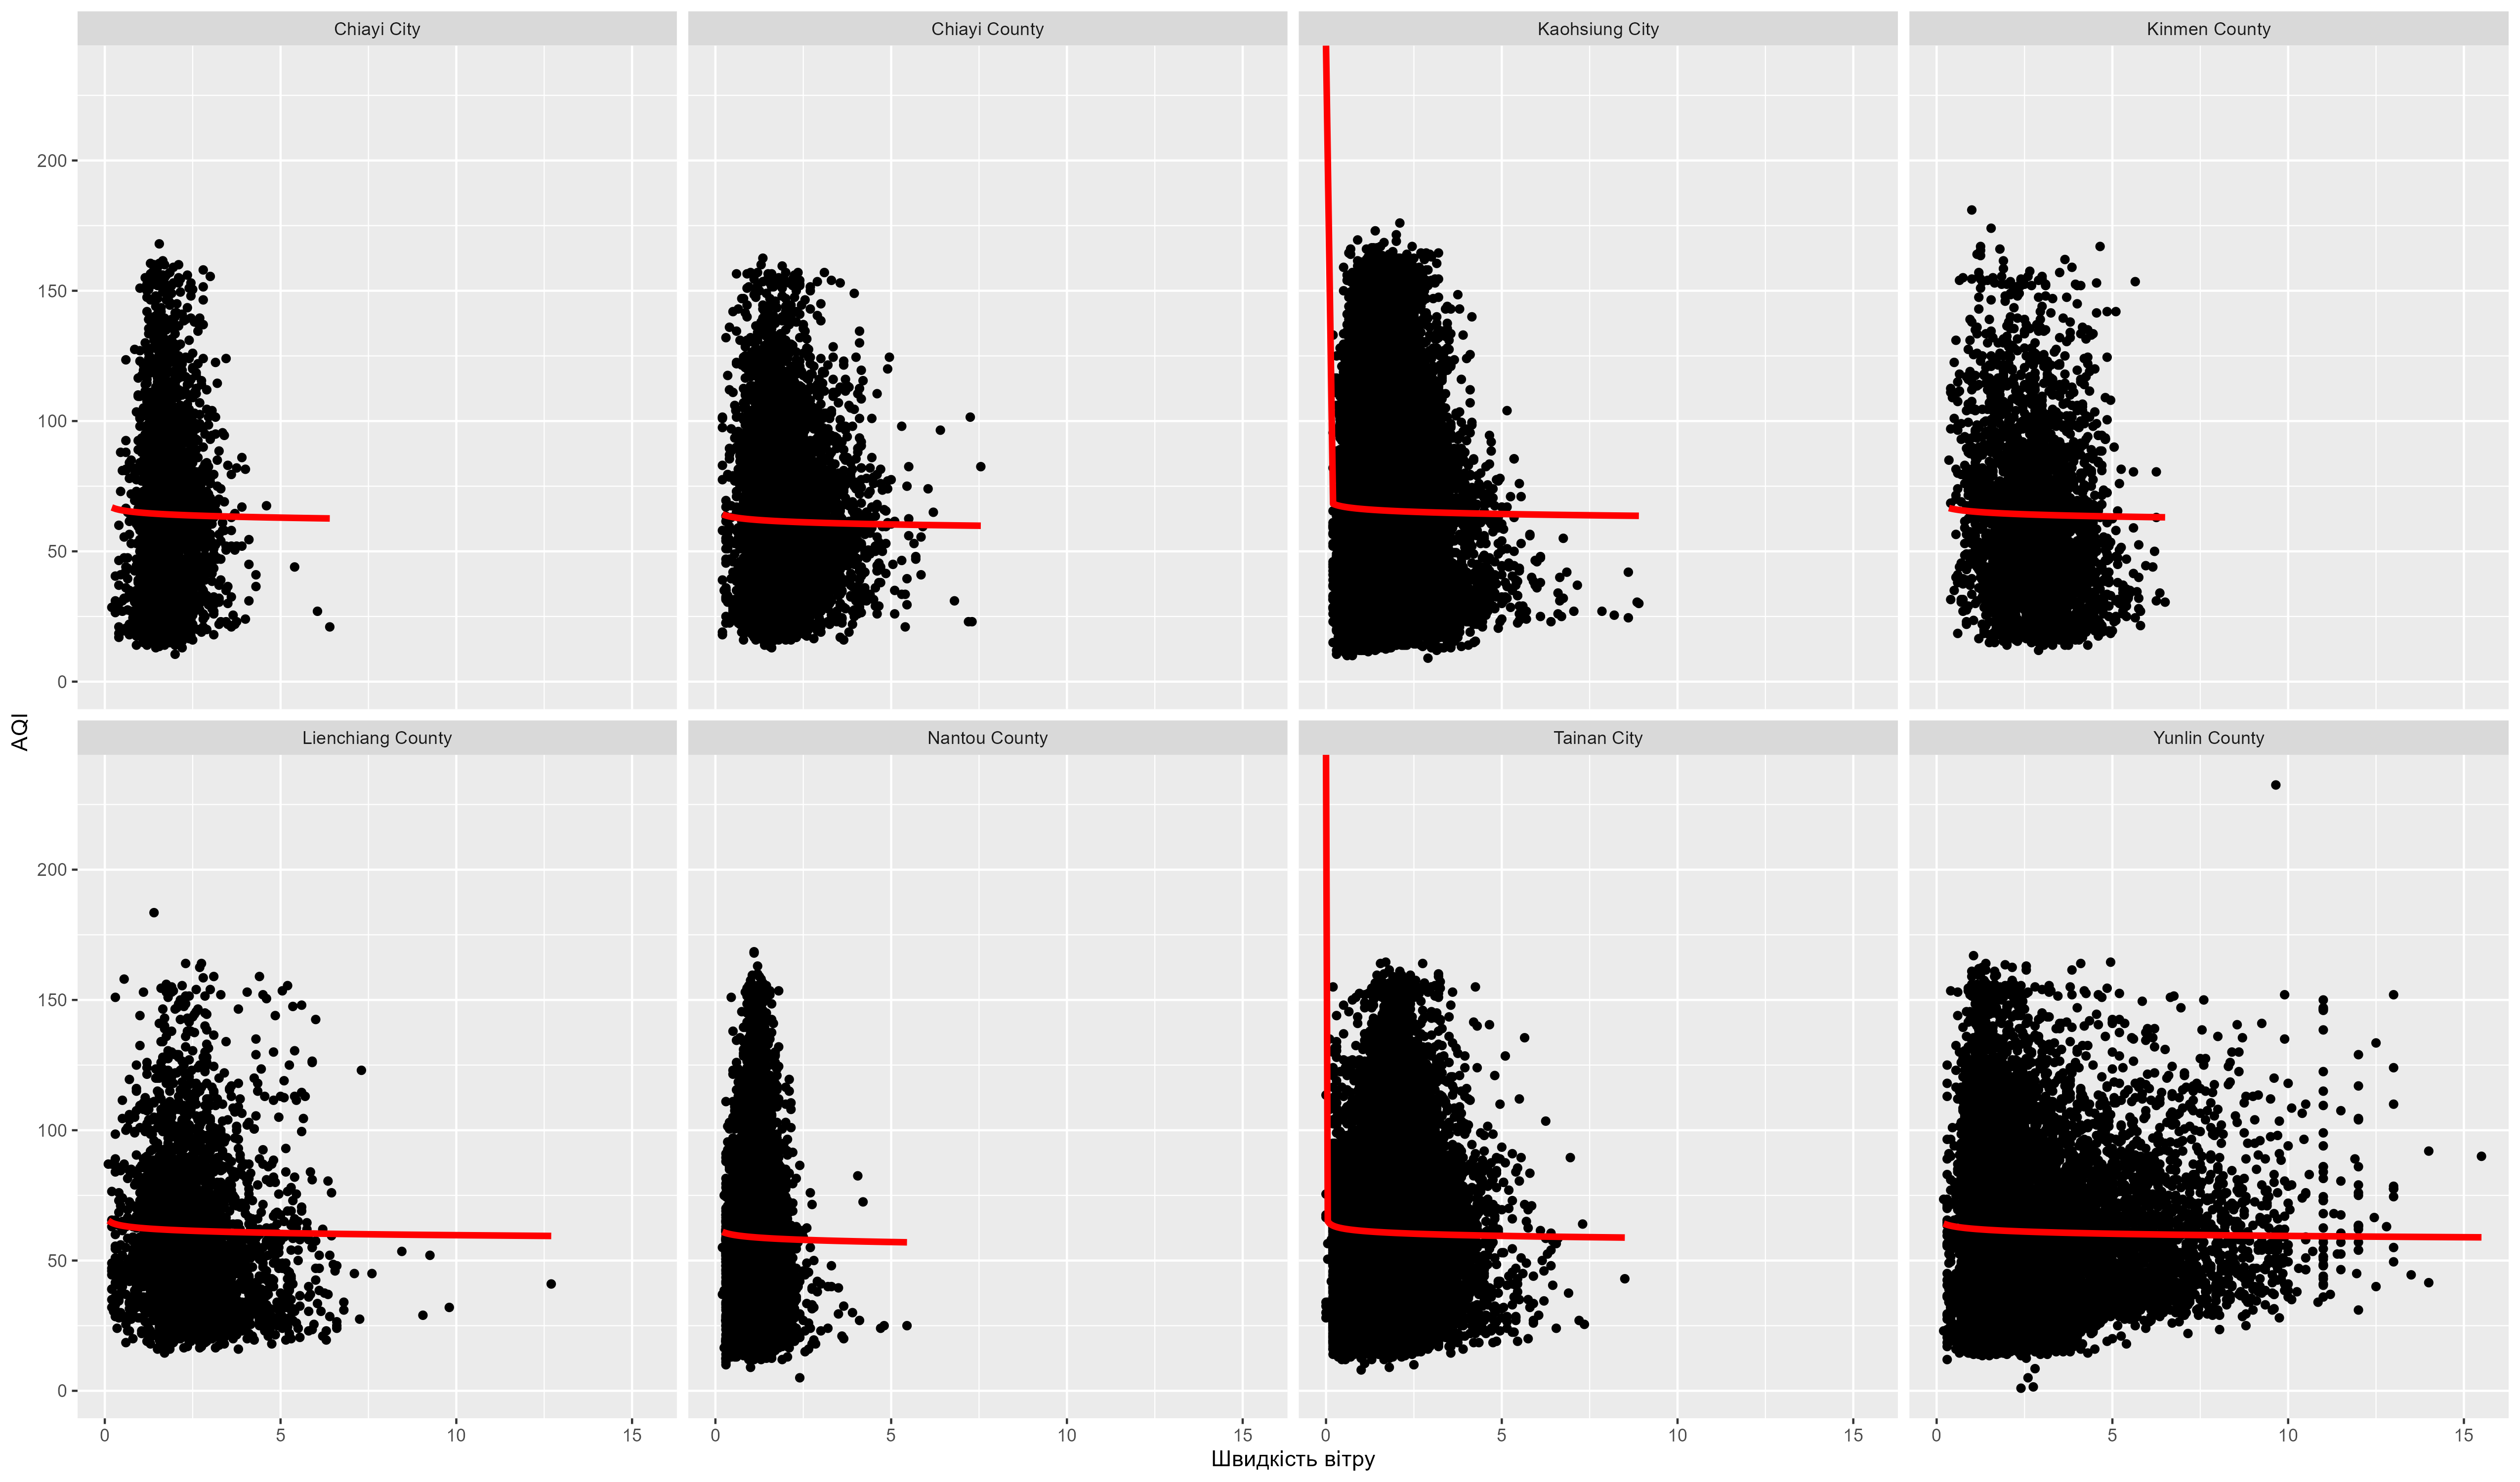
\includegraphics[height=2.5in]{plots/lab3/log(windspeed)-aqi.png}
\end{frame}

\begin{frame}
  \frametitle{Оцінка якості моделей (3)}

  $windspeed^2$:

  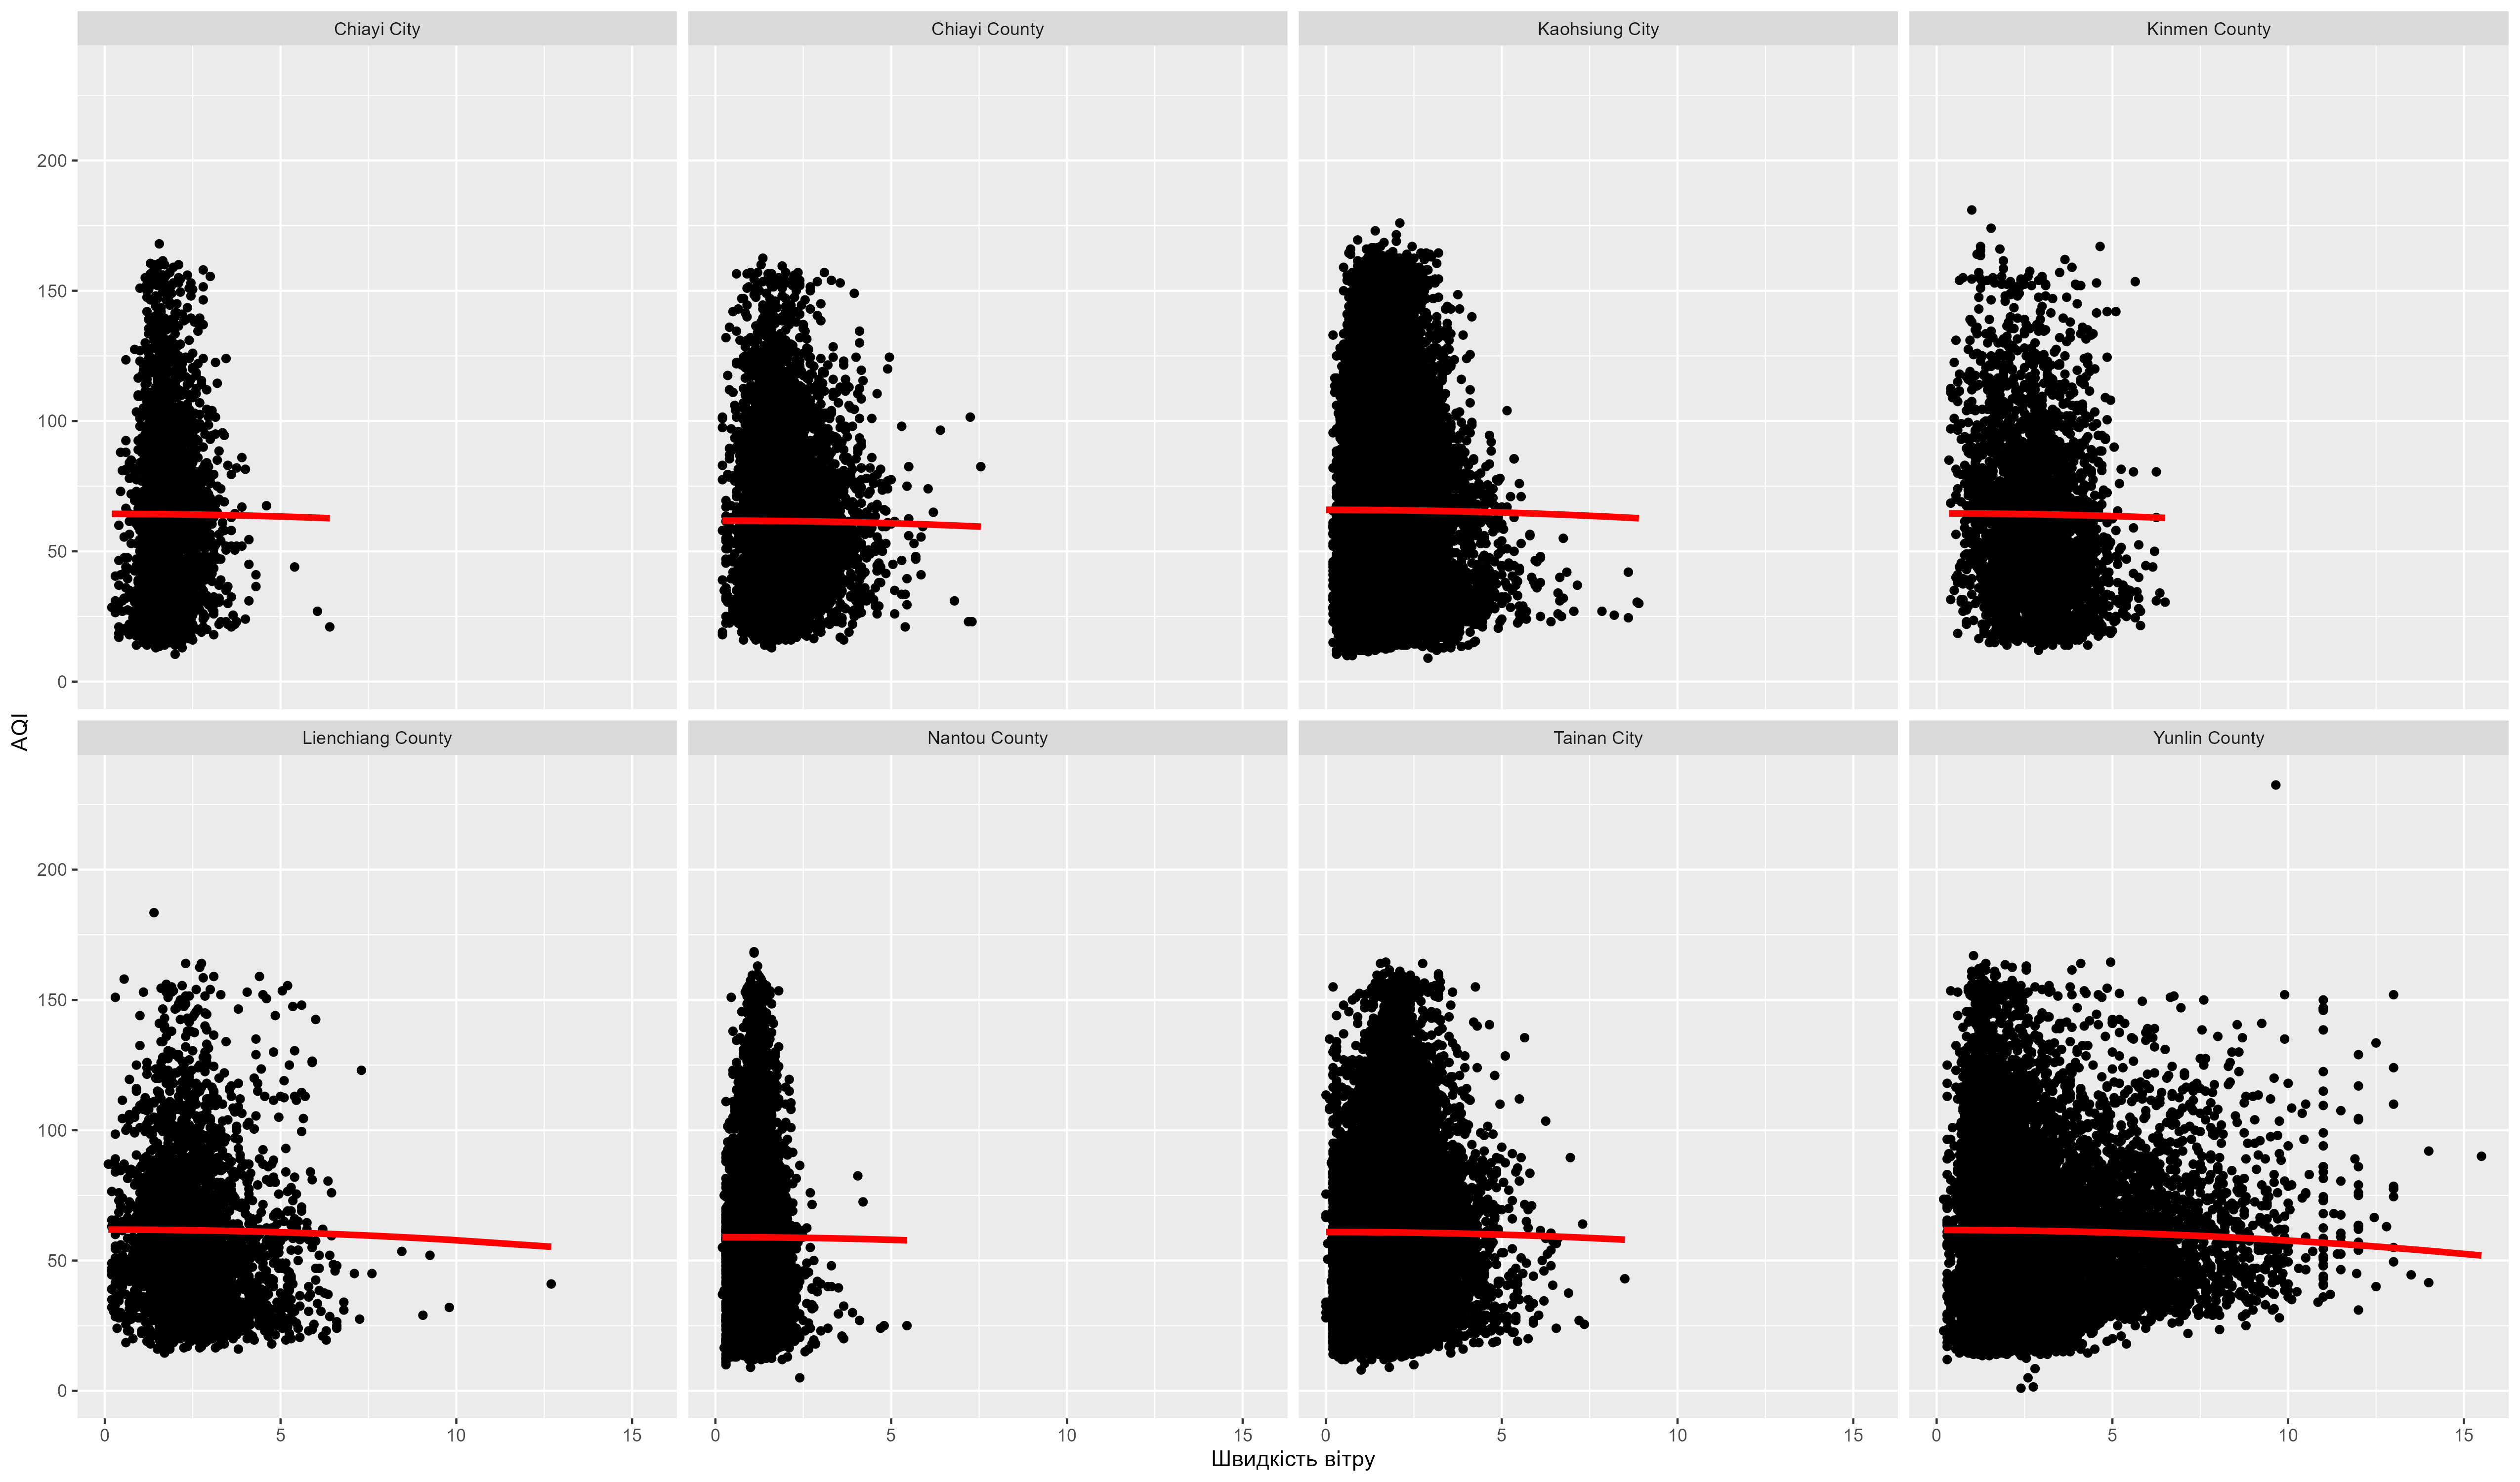
\includegraphics[height=2.5in]{plots/lab3/windspeed^2-aqi.png}
\end{frame}

\begin{frame}
  \frametitle{Оцінка якості моделей (4)}
  
  $windspeed^3$:

  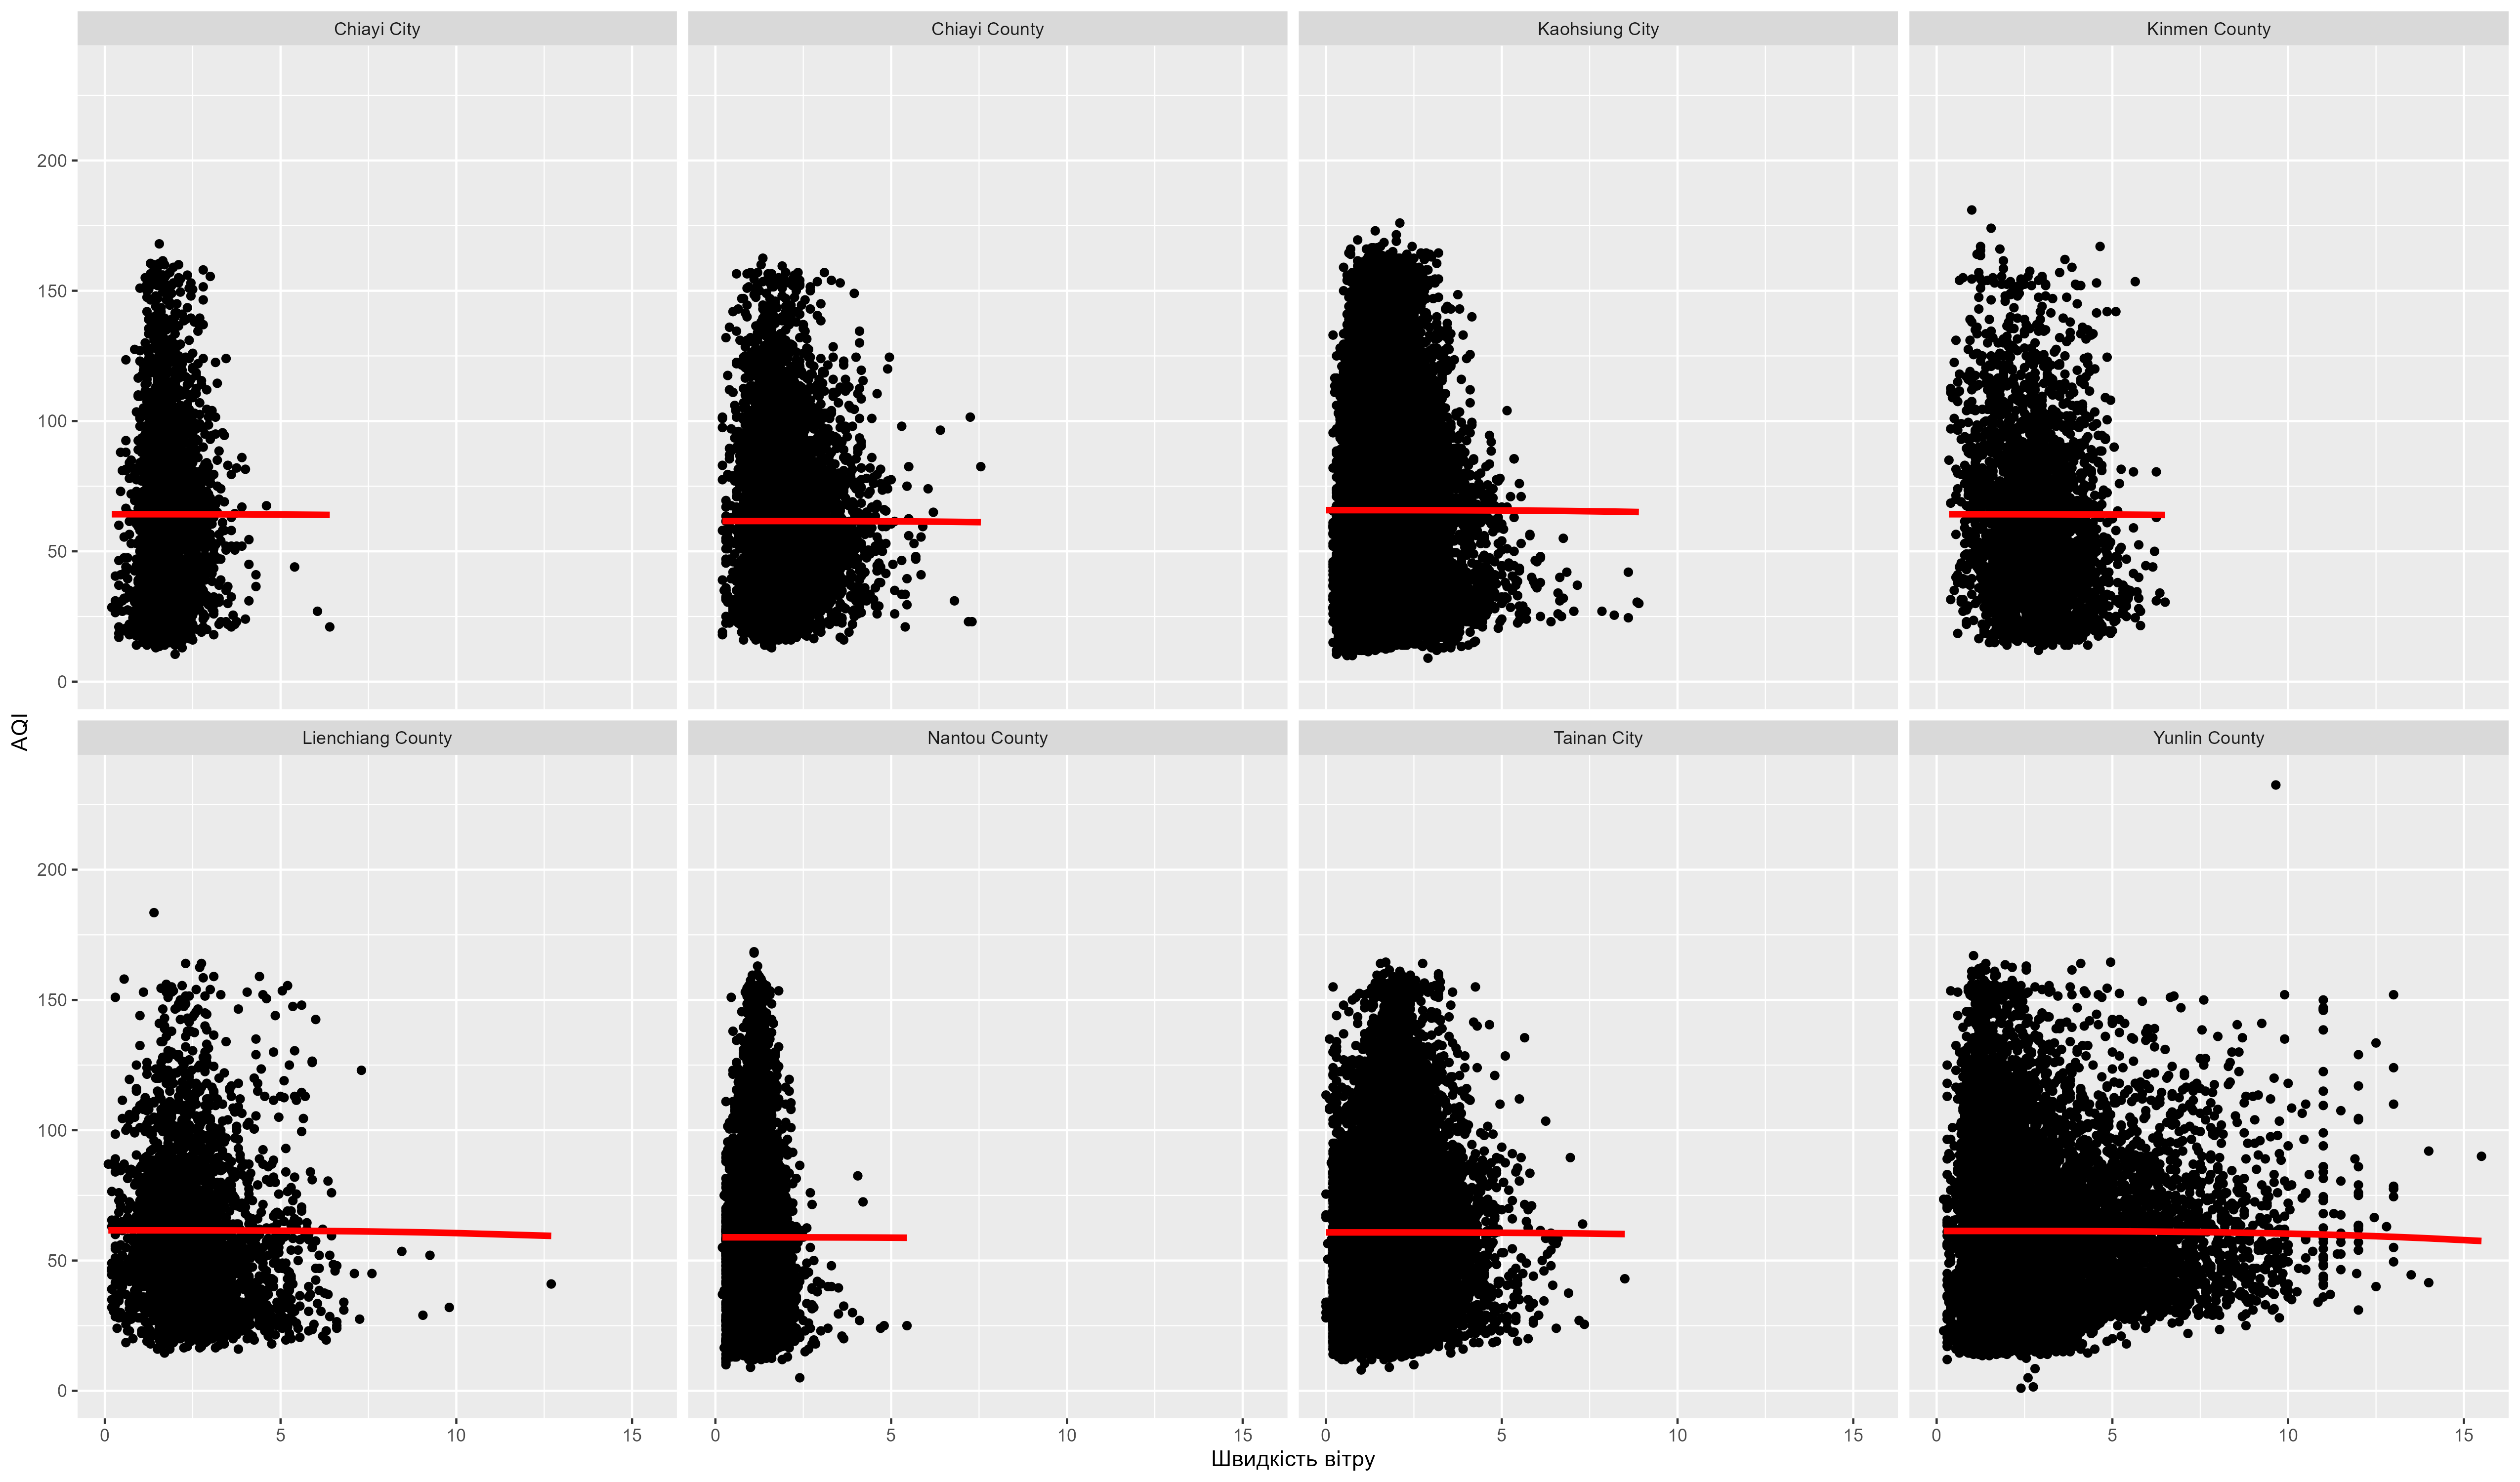
\includegraphics[height=2.5in]{plots/lab3/windspeed^3-aqi.png}
\end{frame}

\begin{frame}
  \frametitle{Оцінка якості моделей (5)}

  \begin{table}
    \centering
    \resizebox{.9\textwidth}{!}{

    \begin{talltblr}[         %% tabularray outer open
    entry=none,label=none,
    note{}={+ p \num{< 0.1}, * p \num{< 0.05}, ** p \num{< 0.01}, *** p \num{< 0.001}},
    ]                     %% tabularray outer close
    {                     %% tabularray inner open
    colspec={Q[]Q[]Q[]Q[]Q[]},
    column{2,3,4,5}={}{halign=c,},
    column{1}={}{halign=l,},
    hline{12}={1,2,3,4,5}{solid, black, 0.05em},
    }                     %% tabularray inner close
    \toprule
    & 1 & 2 & 3 & 4 \\ \midrule %% TinyTableHeader
    after\_reformTRUE & \num{-12.487}*** & \num{-12.581}*** & \num{-12.358}*** & \num{-12.313}*** \\
    & (\num{1.082}) & (\num{1.032}) & (\num{1.089}) & (\num{1.085}) \\
    windspeed & \num{-0.780} &  &  &  \\
    & (\num{0.574}) &  &  &  \\
    log(windspeed) &  & \num{-1.799} &  &  \\
    &  & (\num{1.367}) &  &  \\
    I(windspeed\textasciicircum{}2) &  &  & \num{-0.050} &  \\
    &  &  & (\num{0.064}) &  \\
    I(windspeed\textasciicircum{}3) &  &  &  & \num{-0.001} \\
    &  &  &  & (\num{0.005}) \\
    Num.Obs. & \num{221582} & \num{221339} & \num{221582} & \num{221582} \\
    R2 & \num{0.134} & \num{0.134} & \num{0.133} & \num{0.132} \\
    R2 Adj. & \num{0.134} & \num{0.133} & \num{0.133} & \num{0.132} \\
    \bottomrule
    \end{talltblr}
    }
  \end{table}
\end{frame}

\begin{frame}
  \frametitle{Перевірка на значущість}

  Перевіримо гіпотези на значущість:

  \begin{center}
    \begin{tabular}{cc}
      \hline
      Гіпотеза & p-value \\
      \hline
      after\_reform & $2\cdot10^{-16}$ \\
      windspeed    & 0.1739 \\
    \end{tabular}
  \end{center}

  Отже, можемо прибрати windspeed з моделі.
\end{frame}

\begin{frame}
  \frametitle{Кінцева модель}
   
  \begin{table}
    \centering
    \begin{talltblr}[         %% tabularray outer open
    entry=none,label=none,
    note{}={+ p \num{< 0.1}, * p \num{< 0.05}, ** p \num{< 0.01}, *** p \num{< 0.001}},
    ]                     %% tabularray outer close
    {                     %% tabularray inner open
    colspec={Q[]Q[]},
    column{2}={}{halign=c,},
    column{1}={}{halign=l,},
    hline{4}={1,2}{solid, black, 0.05em},
    }                     %% tabularray inner close
    \toprule
    & Model \\ \midrule %% TinyTableHeader
    after\_reformTRUE & \num{-11.736}*** \\
    & (\num{0.700}) \\
    Num.Obs. & \num{231364} \\
    R2 & \num{0.152} \\
    R2 Adj. & \num{0.151} \\
    \bottomrule
    \end{talltblr}
  \end{table}
\end{frame}

\begin{frame}
  \frametitle{Інтерпретація}
   
\end{frame}

\begin{frame}
  \section{Висновок}

  \frametitle{Зміст}
  \tableofcontents[currentsection]
\end{frame}

\begin{frame}
  \frametitle{Висновок}
   
\end{frame}
\end{document}